%!TEX root=/Users/sergej/Documents/Master/Thesis/main.tex 
\section{Ranking of structural Ricardian comparative advantage }
In this section I present the results of the structural RCA ranking for both value-added exports measures and gross exports. First, I will first focus on the global view by highlighting the results of the association of the RCA ranking for gross exports and value-added exports against a country's per capita GDP. The hypothesis I focus is that country's with a higher GDP show a higher similarity between the rankings. Moreover, poorer countries production structure is such that sourcing and factor usage are more sector specific. \par Second, I will view at the structural RCA results by comparing the rankings for Belgium and Germany of forward and backward value-added exports to gross exports. In this way, I analyze whether two aspects, first whether value-added exports alter the picture of comparative advantage and whether the different perspectives of value-added exports show affect the results. 
\subsection{Structural Ricardian comparative advantage based gross exports and value-added exports}
I will discuss the choice of the association measures shortly. First, I chose the Spearman's $\rho$  since I focus on the similarity of rankings and the strength of the monotonic association between them. Moreover I chose Kendall's $\tau$ as it computes the similarity of the two rankings, by the means of counting the number of country pairs, which are different between two rankings.% Concretely, for each draw of country pairs I record in a binary variable, whether the draws are of the same order as in the ordered set. The binary variable is equal to one if the order is the same and zero else. In the next step I compute a simple correlation coefficient on the set of binary variables.     
\par 
I outline the construction of Kendall's $\tau$ based on \textcite{abdi2007kendall}. The outline makes the simple interpretation of Kendall's $\tau$ in terms of probabilities more clear. The basic idea behind the measure is to count the number of different pairs of two sets of ordered  objects, which include the same objects  \textcite{abdi2007kendall}. I illustrate this idea in the context of the RCA rankings.  For two RCA rankings, the measure is based on counting the number of different ordered country pairs, which I denote as $d(P_1, P_2)$, where $P_i \quad i=1,2$ indicates the two set ordered pairs obtained from the country rankings. In the next step, this number is normalized such that is bounded by -1 and 1, where -1 reflect the largest differences and 1 is equal to the smallest difference.  Kendall's $\tau$ is then defined as follows \[ \tau= \frac{1/2 N(N-1) - d(P_1,P_2)} {1/2 N(N-1)} \], %where the nominator $1/2 N(N-1)$ is equal to the number of pairs one can obtain from a set of $n$ objects. 
Moreover, Kendall's $\tau$ has an intuitive stochastic interpretation based on the idea of drawing orderd pairs \parencite{abdi2007kendall}. In the context of two country rankings, the interpretation is that if a country pair is randomly drawn from each ranking, Kendall's $\tau$ is the difference between the probability that the draws have the same order and the probability that the country pairs have a different order. The focus of Kendall's $\tau$ on country pairs is especially useful  for RCA, as the main focus of RCA is to compare the comparative advantage between pairs of countries and industries.   \par 
\begin{figure}[H]
\caption{Association RCA based on VAX \& EXGR and GDP per capita }
\centering
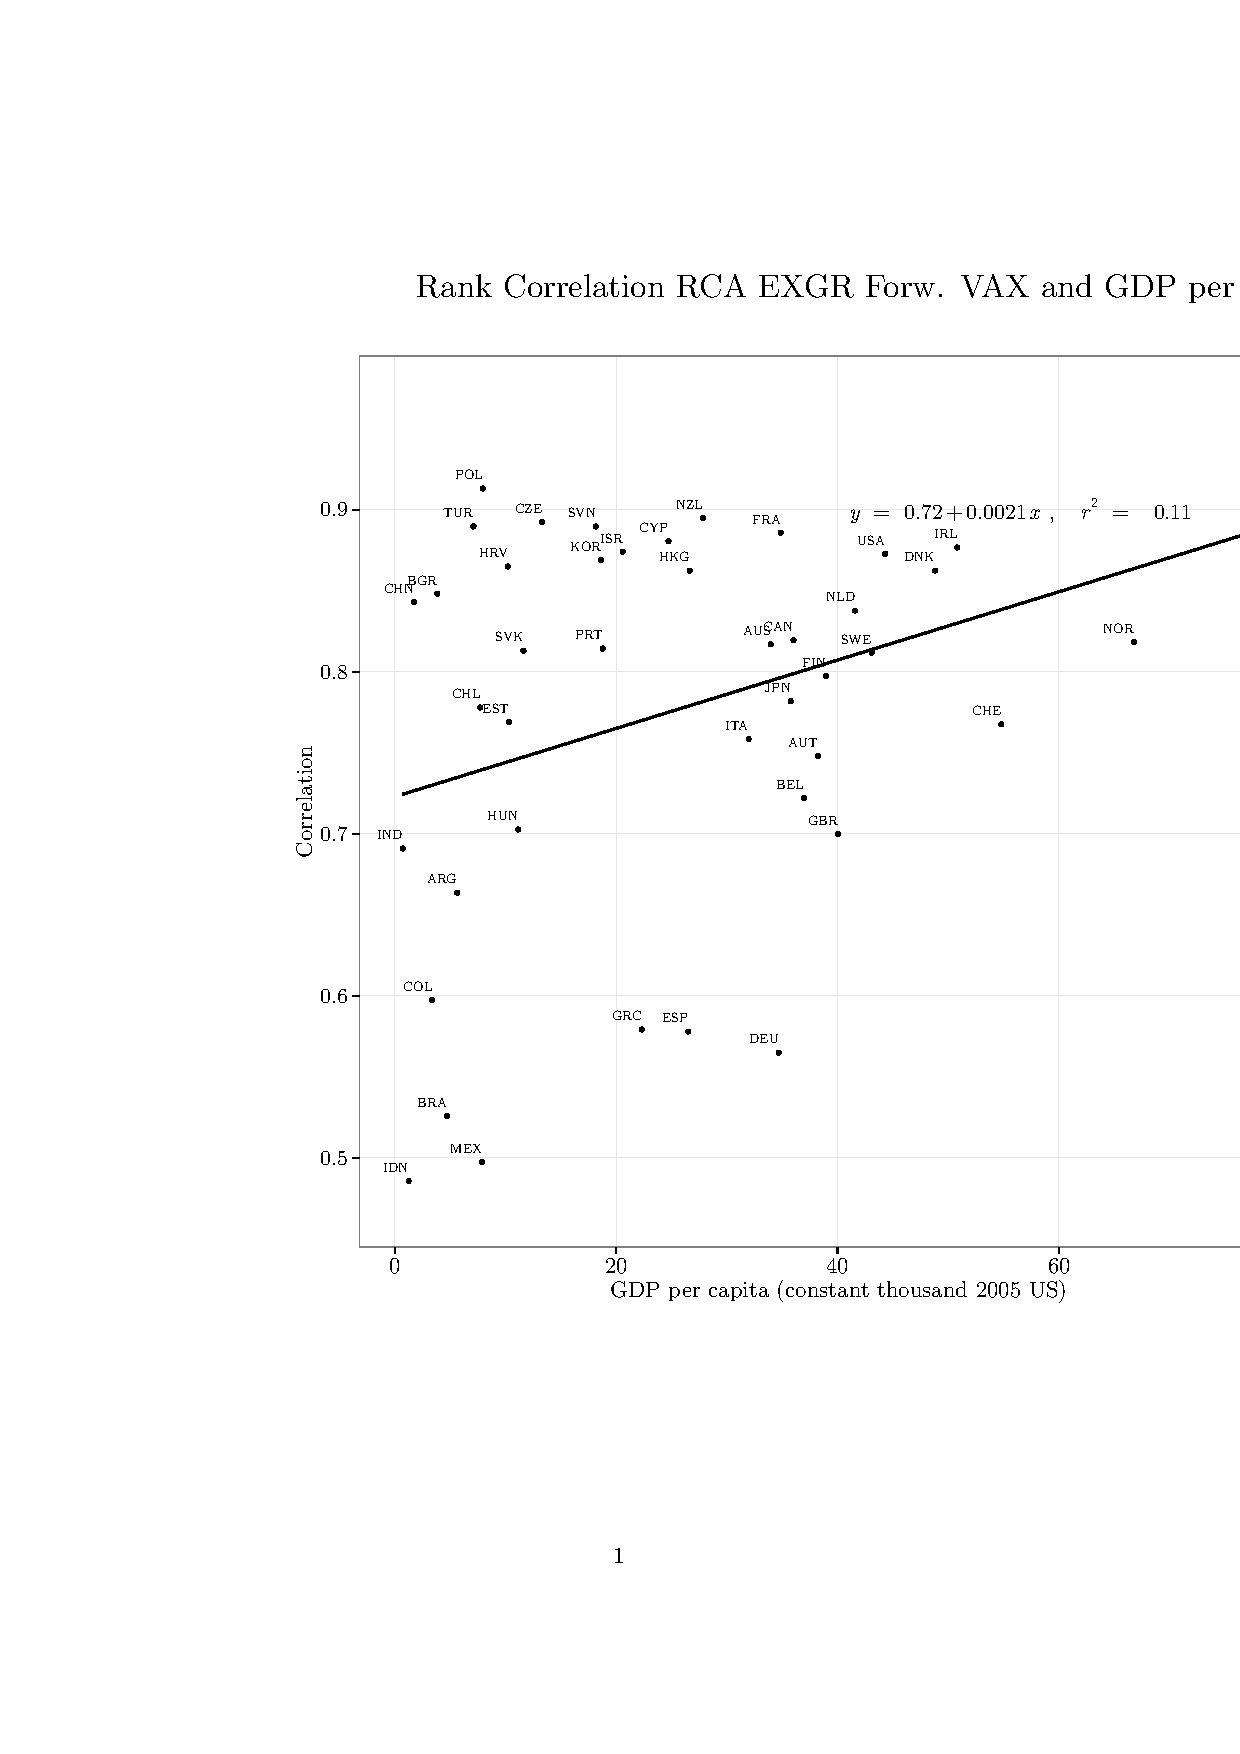
\includegraphics[width=.49 \linewidth]{./fig/spearman_fddva_std_balassa-march.tex}
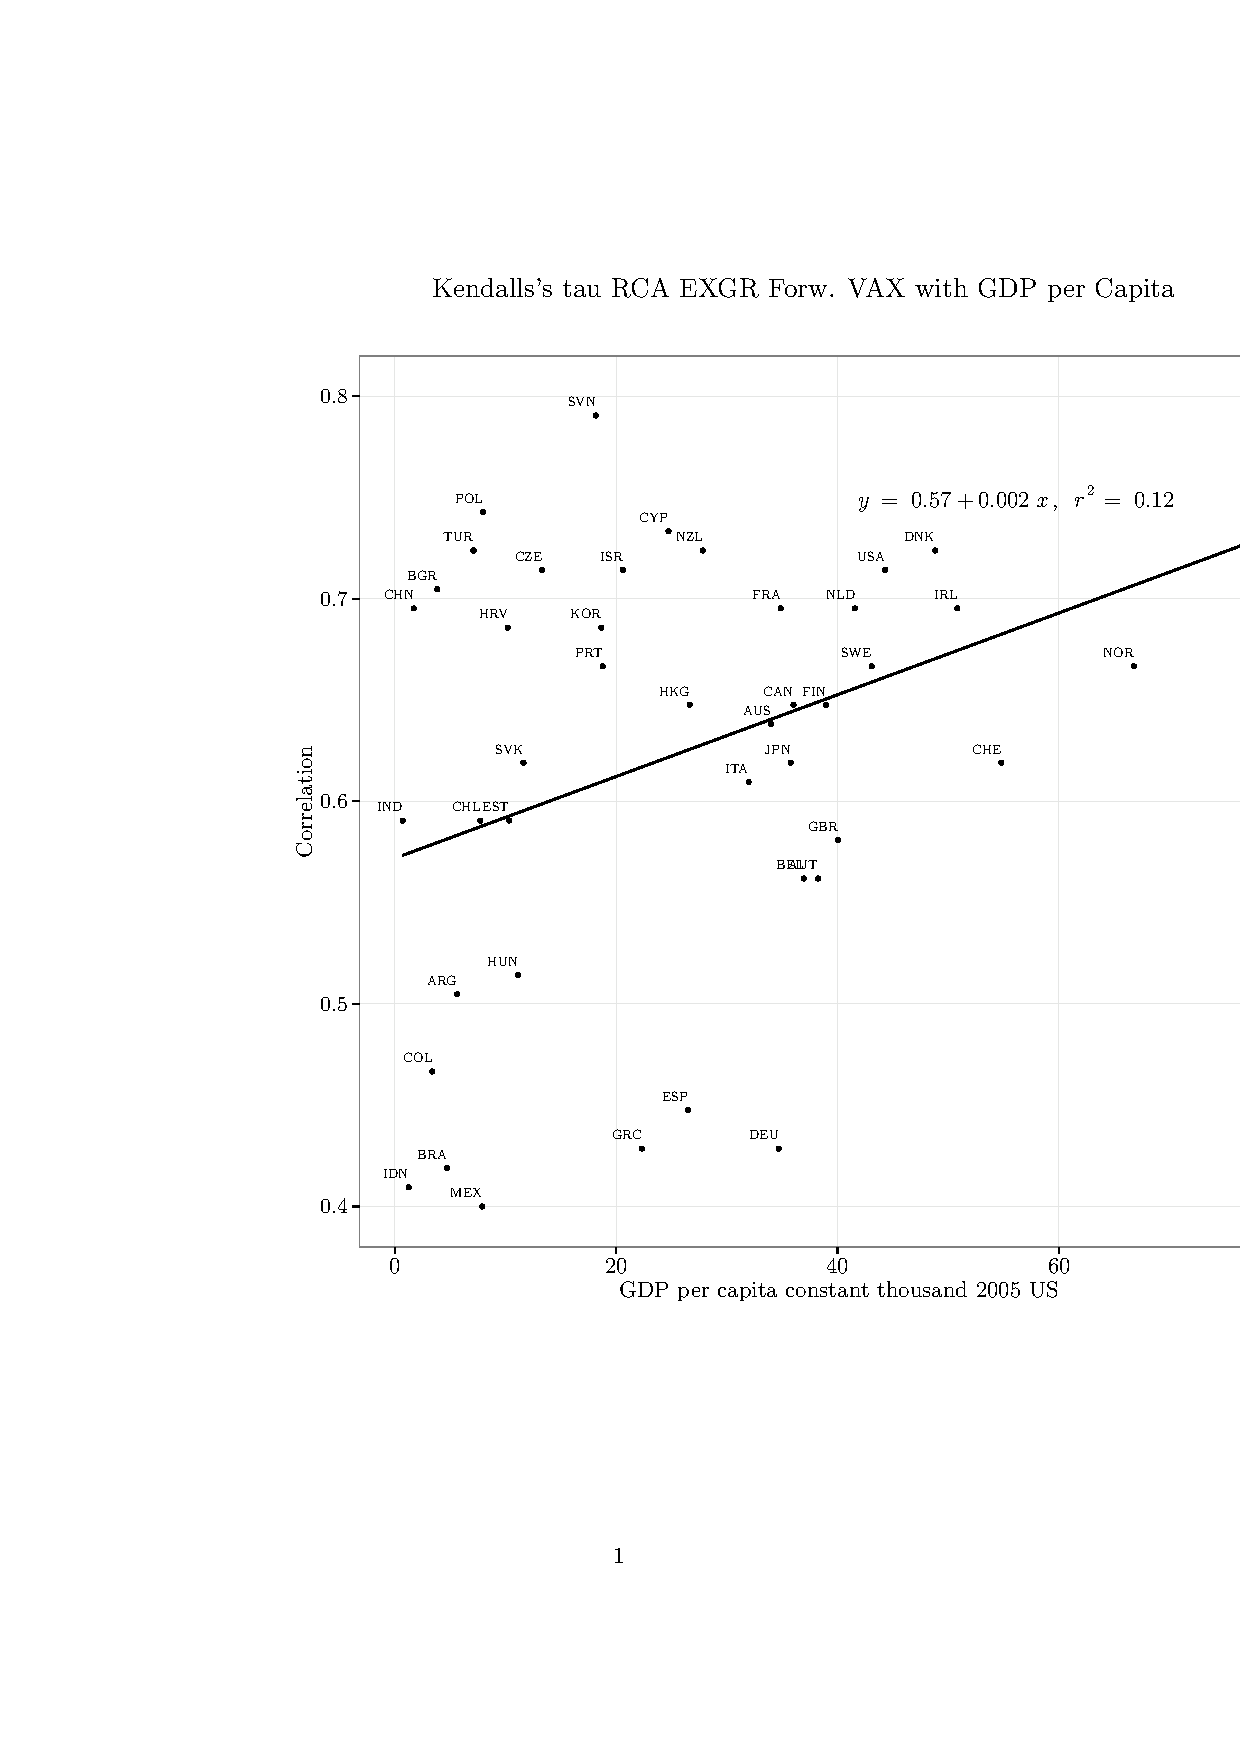
\includegraphics[width=.49\linewidth]{./fig/kendall_fddva_exgr_std_balassa-march.tex}
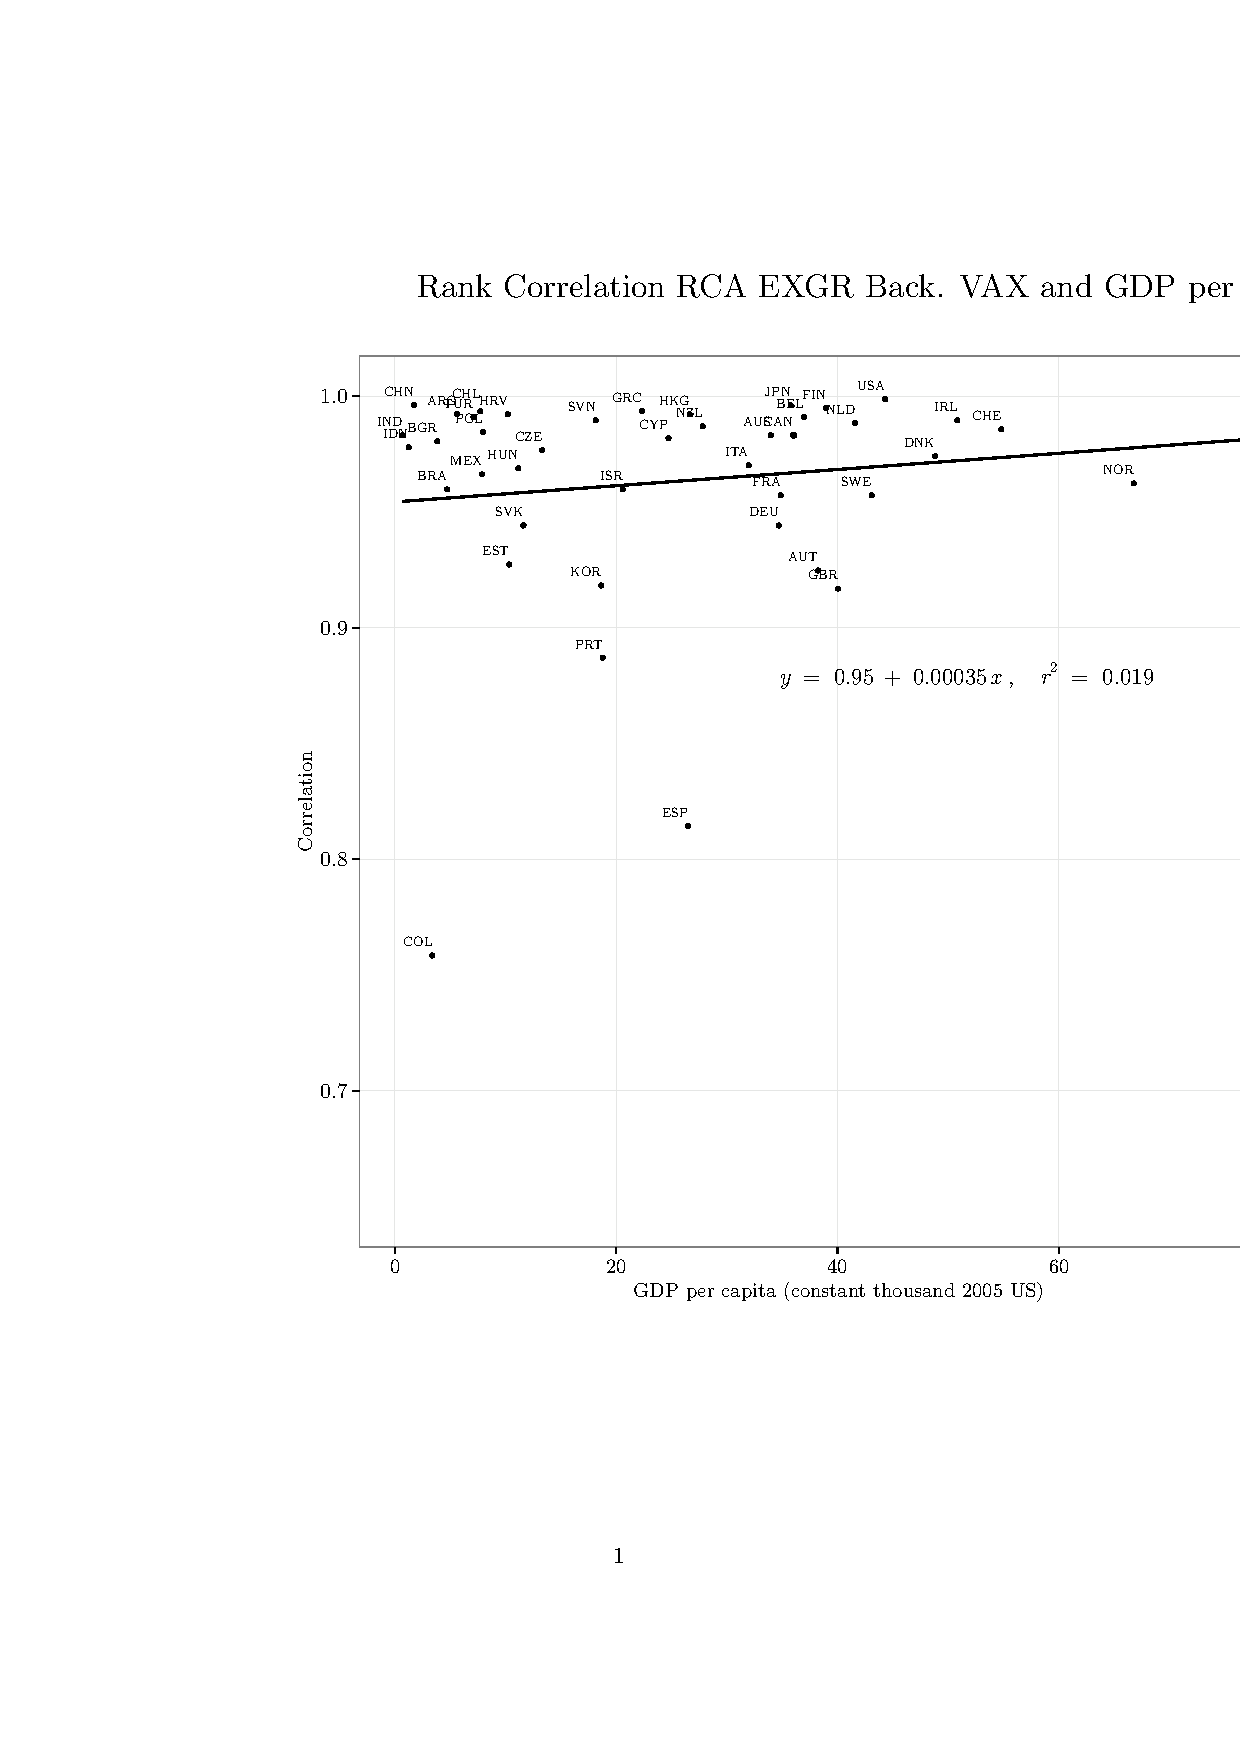
\includegraphics[width=.49 \linewidth]{./fig/spearman_exgr_dva_std_balassa-march.tex}
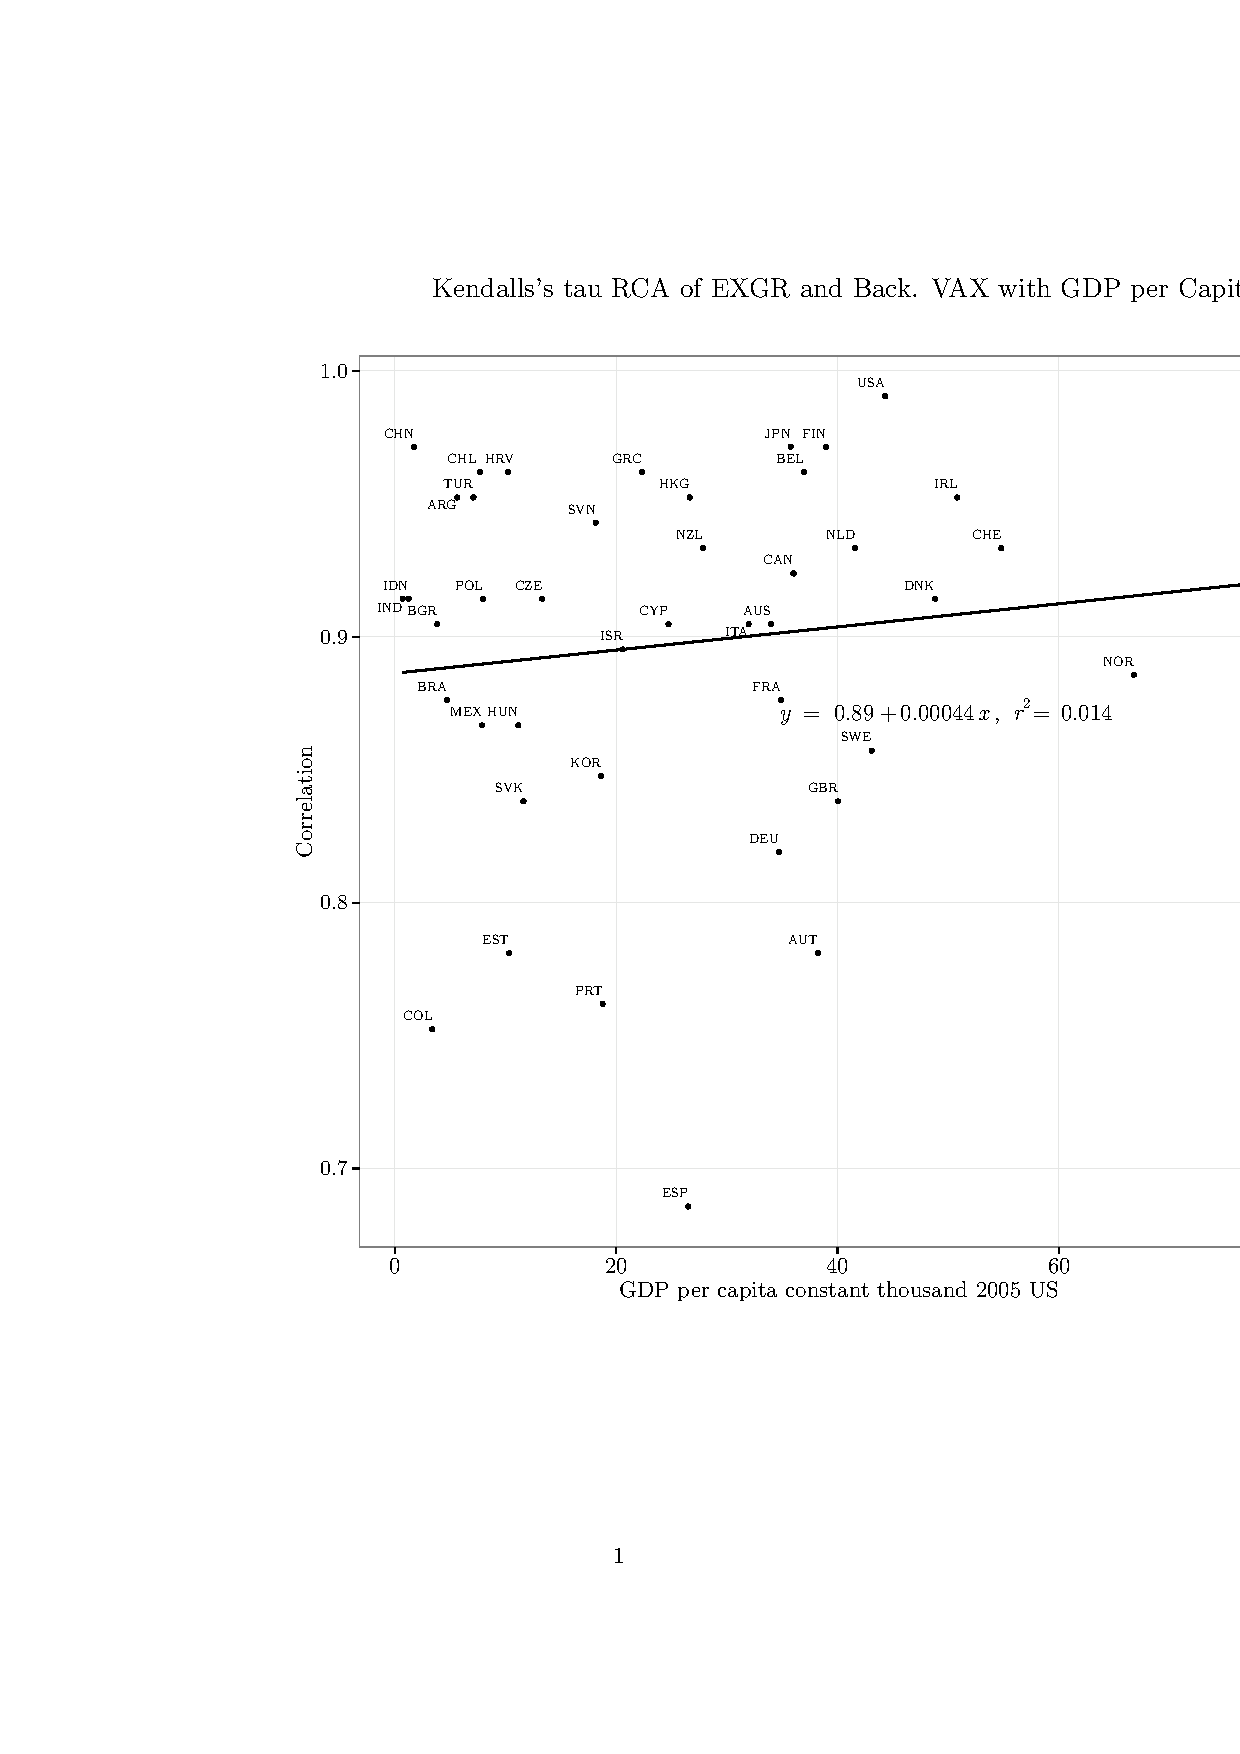
\includegraphics[width=.49\linewidth]{./fig/kendall_dva_exgr_std_balassa-march.tex}
 %\captionof{figure}{Another figure}
\end{figure}
I conclude four findings from the figures above. First, the RCA rankings based on gross exports and backward value-added exports show a high degree of similarity for all countries. Second, the association between forward value-added exports and gross exports is substantially lower than the association of backward value-added and gross exports. Third,  the association of gross exports and forw. VAX shows a weak positive relation with a country's GDP per capita. Fourth, overall the strenght of association as measured by Spearman's $\rho$ is higher than Kendall's $\tau$. \par The first and second finding are similar to the results in the estimation of the $\theta$ parameter. The results showed that the estimates for backw. VAX and gross exports showed a similar pattern, while the estimates of forw. VAX were reduced and did not follow a pattern. The third finding is consistent with the hypothesis that countries with a higher GDP have less sector specific input and sourcing patterns. The forth finding is consistent with the result that asymptotically the ratio of the population analog of Spearman's $\rho$ and Kendall's $\tau$ is equal to three half \parencite{fredricks2007}. \par
Turning to the local view  I present below the normalized RCA based on both value-added export measures and gross exports for the industries of the manufacturing sector.   the RCA \footnote{ Formally, I define it as follows $RCA_{i}^{k}=\frac{ z^k_i * \bar{z} }{\bar{z}_i * \bar{z}^k}$, where $\bar{z}$ denotes the grand mean, $\bar{z}^k$ denotes the sector specific mean and $\bar{z}_i$ denotes the country specific mean.} as in \textcite{leromain2014}, such that a value above 1 indicates a comparative advantage of the country in the particular industry. I will first discuss the results for backward value-added exports and gross exports. \par  The graph shows that both Germany and Belgium have an comparative advantage in the following sectors . Germany has a higher comparative advantage in x sectors namely . On the other hand Belgium has an comparative advantage in y sectors namely . The graph main interesting point to us is that for both countries backward value added closely traces the pattern of gross exports. This results resembles the result of
 the estimation of $\theta$, where I observed a similar picture. \par In contrast, I observe that the RCA ranking are different for forward value-added gross exports. First I observe that 
 \begin{figure}
\caption{Country pair RCA based on for- and backward  VAX \& EXGR }
\includegraphics[width=.5\linewidth]{./fig/forw_exgr_DEU_BEL_tiva.tex}
\includegraphics[width=.5\linewidth]{./fig/back_exgr_DEU_BEL_tiva.tex}
\end{figure}

\endinput